\documentclass{article} % For LaTeX2e
\usepackage{iclr2027_conference,times}

% Optional math commands from https://github.com/goodfeli/dlbook_notation.
%%%%% NEW MATH DEFINITIONS %%%%%

\usepackage{amsmath,amsfonts,bm}

% Mark sections of captions for referring to divisions of figures
\newcommand{\figleft}{{\em (Left)}}
\newcommand{\figcenter}{{\em (Center)}}
\newcommand{\figright}{{\em (Right)}}
\newcommand{\figtop}{{\em (Top)}}
\newcommand{\figbottom}{{\em (Bottom)}}
\newcommand{\captiona}{{\em (a)}}
\newcommand{\captionb}{{\em (b)}}
\newcommand{\captionc}{{\em (c)}}
\newcommand{\captiond}{{\em (d)}}

% Highlight a newly defined term
\newcommand{\newterm}[1]{{\bf #1}}


% Figure reference, lower-case.
\def\figref#1{figure~\ref{#1}}
% Figure reference, capital. For start of sentence
\def\Figref#1{Figure~\ref{#1}}
\def\twofigref#1#2{figures \ref{#1} and \ref{#2}}
\def\quadfigref#1#2#3#4{figures \ref{#1}, \ref{#2}, \ref{#3} and \ref{#4}}
% Section reference, lower-case.
\def\secref#1{section~\ref{#1}}
% Section reference, capital.
\def\Secref#1{Section~\ref{#1}}
% Reference to two sections.
\def\twosecrefs#1#2{sections \ref{#1} and \ref{#2}}
% Reference to three sections.
\def\secrefs#1#2#3{sections \ref{#1}, \ref{#2} and \ref{#3}}
% Reference to an equation, lower-case.
\def\eqref#1{equation~\ref{#1}}
% Reference to an equation, upper case
\def\Eqref#1{Equation~\ref{#1}}
% A raw reference to an equation---avoid using if possible
\def\plaineqref#1{\ref{#1}}
% Reference to a chapter, lower-case.
\def\chapref#1{chapter~\ref{#1}}
% Reference to an equation, upper case.
\def\Chapref#1{Chapter~\ref{#1}}
% Reference to a range of chapters
\def\rangechapref#1#2{chapters\ref{#1}--\ref{#2}}
% Reference to an algorithm, lower-case.
\def\algref#1{algorithm~\ref{#1}}
% Reference to an algorithm, upper case.
\def\Algref#1{Algorithm~\ref{#1}}
\def\twoalgref#1#2{algorithms \ref{#1} and \ref{#2}}
\def\Twoalgref#1#2{Algorithms \ref{#1} and \ref{#2}}
% Reference to a part, lower case
\def\partref#1{part~\ref{#1}}
% Reference to a part, upper case
\def\Partref#1{Part~\ref{#1}}
\def\twopartref#1#2{parts \ref{#1} and \ref{#2}}

\def\ceil#1{\lceil #1 \rceil}
\def\floor#1{\lfloor #1 \rfloor}
\def\1{\bm{1}}
\newcommand{\train}{\mathcal{D}}
\newcommand{\valid}{\mathcal{D_{\mathrm{valid}}}}
\newcommand{\test}{\mathcal{D_{\mathrm{test}}}}

\def\eps{{\epsilon}}


% Random variables
\def\reta{{\textnormal{$\eta$}}}
\def\ra{{\textnormal{a}}}
\def\rb{{\textnormal{b}}}
\def\rc{{\textnormal{c}}}
\def\rd{{\textnormal{d}}}
\def\re{{\textnormal{e}}}
\def\rf{{\textnormal{f}}}
\def\rg{{\textnormal{g}}}
\def\rh{{\textnormal{h}}}
\def\ri{{\textnormal{i}}}
\def\rj{{\textnormal{j}}}
\def\rk{{\textnormal{k}}}
\def\rl{{\textnormal{l}}}
% rm is already a command, just don't name any random variables m
\def\rn{{\textnormal{n}}}
\def\ro{{\textnormal{o}}}
\def\rp{{\textnormal{p}}}
\def\rq{{\textnormal{q}}}
\def\rr{{\textnormal{r}}}
\def\rs{{\textnormal{s}}}
\def\rt{{\textnormal{t}}}
\def\ru{{\textnormal{u}}}
\def\rv{{\textnormal{v}}}
\def\rw{{\textnormal{w}}}
\def\rx{{\textnormal{x}}}
\def\ry{{\textnormal{y}}}
\def\rz{{\textnormal{z}}}

% Random vectors
\def\rvepsilon{{\mathbf{\epsilon}}}
\def\rvtheta{{\mathbf{\theta}}}
\def\rva{{\mathbf{a}}}
\def\rvb{{\mathbf{b}}}
\def\rvc{{\mathbf{c}}}
\def\rvd{{\mathbf{d}}}
\def\rve{{\mathbf{e}}}
\def\rvf{{\mathbf{f}}}
\def\rvg{{\mathbf{g}}}
\def\rvh{{\mathbf{h}}}
\def\rvu{{\mathbf{i}}}
\def\rvj{{\mathbf{j}}}
\def\rvk{{\mathbf{k}}}
\def\rvl{{\mathbf{l}}}
\def\rvm{{\mathbf{m}}}
\def\rvn{{\mathbf{n}}}
\def\rvo{{\mathbf{o}}}
\def\rvp{{\mathbf{p}}}
\def\rvq{{\mathbf{q}}}
\def\rvr{{\mathbf{r}}}
\def\rvs{{\mathbf{s}}}
\def\rvt{{\mathbf{t}}}
\def\rvu{{\mathbf{u}}}
\def\rvv{{\mathbf{v}}}
\def\rvw{{\mathbf{w}}}
\def\rvx{{\mathbf{x}}}
\def\rvy{{\mathbf{y}}}
\def\rvz{{\mathbf{z}}}

% Elements of random vectors
\def\erva{{\textnormal{a}}}
\def\ervb{{\textnormal{b}}}
\def\ervc{{\textnormal{c}}}
\def\ervd{{\textnormal{d}}}
\def\erve{{\textnormal{e}}}
\def\ervf{{\textnormal{f}}}
\def\ervg{{\textnormal{g}}}
\def\ervh{{\textnormal{h}}}
\def\ervi{{\textnormal{i}}}
\def\ervj{{\textnormal{j}}}
\def\ervk{{\textnormal{k}}}
\def\ervl{{\textnormal{l}}}
\def\ervm{{\textnormal{m}}}
\def\ervn{{\textnormal{n}}}
\def\ervo{{\textnormal{o}}}
\def\ervp{{\textnormal{p}}}
\def\ervq{{\textnormal{q}}}
\def\ervr{{\textnormal{r}}}
\def\ervs{{\textnormal{s}}}
\def\ervt{{\textnormal{t}}}
\def\ervu{{\textnormal{u}}}
\def\ervv{{\textnormal{v}}}
\def\ervw{{\textnormal{w}}}
\def\ervx{{\textnormal{x}}}
\def\ervy{{\textnormal{y}}}
\def\ervz{{\textnormal{z}}}

% Random matrices
\def\rmA{{\mathbf{A}}}
\def\rmB{{\mathbf{B}}}
\def\rmC{{\mathbf{C}}}
\def\rmD{{\mathbf{D}}}
\def\rmE{{\mathbf{E}}}
\def\rmF{{\mathbf{F}}}
\def\rmG{{\mathbf{G}}}
\def\rmH{{\mathbf{H}}}
\def\rmI{{\mathbf{I}}}
\def\rmJ{{\mathbf{J}}}
\def\rmK{{\mathbf{K}}}
\def\rmL{{\mathbf{L}}}
\def\rmM{{\mathbf{M}}}
\def\rmN{{\mathbf{N}}}
\def\rmO{{\mathbf{O}}}
\def\rmP{{\mathbf{P}}}
\def\rmQ{{\mathbf{Q}}}
\def\rmR{{\mathbf{R}}}
\def\rmS{{\mathbf{S}}}
\def\rmT{{\mathbf{T}}}
\def\rmU{{\mathbf{U}}}
\def\rmV{{\mathbf{V}}}
\def\rmW{{\mathbf{W}}}
\def\rmX{{\mathbf{X}}}
\def\rmY{{\mathbf{Y}}}
\def\rmZ{{\mathbf{Z}}}

% Elements of random matrices
\def\ermA{{\textnormal{A}}}
\def\ermB{{\textnormal{B}}}
\def\ermC{{\textnormal{C}}}
\def\ermD{{\textnormal{D}}}
\def\ermE{{\textnormal{E}}}
\def\ermF{{\textnormal{F}}}
\def\ermG{{\textnormal{G}}}
\def\ermH{{\textnormal{H}}}
\def\ermI{{\textnormal{I}}}
\def\ermJ{{\textnormal{J}}}
\def\ermK{{\textnormal{K}}}
\def\ermL{{\textnormal{L}}}
\def\ermM{{\textnormal{M}}}
\def\ermN{{\textnormal{N}}}
\def\ermO{{\textnormal{O}}}
\def\ermP{{\textnormal{P}}}
\def\ermQ{{\textnormal{Q}}}
\def\ermR{{\textnormal{R}}}
\def\ermS{{\textnormal{S}}}
\def\ermT{{\textnormal{T}}}
\def\ermU{{\textnormal{U}}}
\def\ermV{{\textnormal{V}}}
\def\ermW{{\textnormal{W}}}
\def\ermX{{\textnormal{X}}}
\def\ermY{{\textnormal{Y}}}
\def\ermZ{{\textnormal{Z}}}

% Vectors
\def\vzero{{\bm{0}}}
\def\vone{{\bm{1}}}
\def\vmu{{\bm{\mu}}}
\def\vtheta{{\bm{\theta}}}
\def\va{{\bm{a}}}
\def\vb{{\bm{b}}}
\def\vc{{\bm{c}}}
\def\vd{{\bm{d}}}
\def\ve{{\bm{e}}}
\def\vf{{\bm{f}}}
\def\vg{{\bm{g}}}
\def\vh{{\bm{h}}}
\def\vi{{\bm{i}}}
\def\vj{{\bm{j}}}
\def\vk{{\bm{k}}}
\def\vl{{\bm{l}}}
\def\vm{{\bm{m}}}
\def\vn{{\bm{n}}}
\def\vo{{\bm{o}}}
\def\vp{{\bm{p}}}
\def\vq{{\bm{q}}}
\def\vr{{\bm{r}}}
\def\vs{{\bm{s}}}
\def\vt{{\bm{t}}}
\def\vu{{\bm{u}}}
\def\vv{{\bm{v}}}
\def\vw{{\bm{w}}}
\def\vx{{\bm{x}}}
\def\vy{{\bm{y}}}
\def\vz{{\bm{z}}}

% Elements of vectors
\def\evalpha{{\alpha}}
\def\evbeta{{\beta}}
\def\evepsilon{{\epsilon}}
\def\evlambda{{\lambda}}
\def\evomega{{\omega}}
\def\evmu{{\mu}}
\def\evpsi{{\psi}}
\def\evsigma{{\sigma}}
\def\evtheta{{\theta}}
\def\eva{{a}}
\def\evb{{b}}
\def\evc{{c}}
\def\evd{{d}}
\def\eve{{e}}
\def\evf{{f}}
\def\evg{{g}}
\def\evh{{h}}
\def\evi{{i}}
\def\evj{{j}}
\def\evk{{k}}
\def\evl{{l}}
\def\evm{{m}}
\def\evn{{n}}
\def\evo{{o}}
\def\evp{{p}}
\def\evq{{q}}
\def\evr{{r}}
\def\evs{{s}}
\def\evt{{t}}
\def\evu{{u}}
\def\evv{{v}}
\def\evw{{w}}
\def\evx{{x}}
\def\evy{{y}}
\def\evz{{z}}

% Matrix
\def\mA{{\bm{A}}}
\def\mB{{\bm{B}}}
\def\mC{{\bm{C}}}
\def\mD{{\bm{D}}}
\def\mE{{\bm{E}}}
\def\mF{{\bm{F}}}
\def\mG{{\bm{G}}}
\def\mH{{\bm{H}}}
\def\mI{{\bm{I}}}
\def\mJ{{\bm{J}}}
\def\mK{{\bm{K}}}
\def\mL{{\bm{L}}}
\def\mM{{\bm{M}}}
\def\mN{{\bm{N}}}
\def\mO{{\bm{O}}}
\def\mP{{\bm{P}}}
\def\mQ{{\bm{Q}}}
\def\mR{{\bm{R}}}
\def\mS{{\bm{S}}}
\def\mT{{\bm{T}}}
\def\mU{{\bm{U}}}
\def\mV{{\bm{V}}}
\def\mW{{\bm{W}}}
\def\mX{{\bm{X}}}
\def\mY{{\bm{Y}}}
\def\mZ{{\bm{Z}}}
\def\mBeta{{\bm{\beta}}}
\def\mPhi{{\bm{\Phi}}}
\def\mLambda{{\bm{\Lambda}}}
\def\mSigma{{\bm{\Sigma}}}

% Tensor
\DeclareMathAlphabet{\mathsfit}{\encodingdefault}{\sfdefault}{m}{sl}
\SetMathAlphabet{\mathsfit}{bold}{\encodingdefault}{\sfdefault}{bx}{n}
\newcommand{\tens}[1]{\bm{\mathsfit{#1}}}
\def\tA{{\tens{A}}}
\def\tB{{\tens{B}}}
\def\tC{{\tens{C}}}
\def\tD{{\tens{D}}}
\def\tE{{\tens{E}}}
\def\tF{{\tens{F}}}
\def\tG{{\tens{G}}}
\def\tH{{\tens{H}}}
\def\tI{{\tens{I}}}
\def\tJ{{\tens{J}}}
\def\tK{{\tens{K}}}
\def\tL{{\tens{L}}}
\def\tM{{\tens{M}}}
\def\tN{{\tens{N}}}
\def\tO{{\tens{O}}}
\def\tP{{\tens{P}}}
\def\tQ{{\tens{Q}}}
\def\tR{{\tens{R}}}
\def\tS{{\tens{S}}}
\def\tT{{\tens{T}}}
\def\tU{{\tens{U}}}
\def\tV{{\tens{V}}}
\def\tW{{\tens{W}}}
\def\tX{{\tens{X}}}
\def\tY{{\tens{Y}}}
\def\tZ{{\tens{Z}}}


% Graph
\def\gA{{\mathcal{A}}}
\def\gB{{\mathcal{B}}}
\def\gC{{\mathcal{C}}}
\def\gD{{\mathcal{D}}}
\def\gE{{\mathcal{E}}}
\def\gF{{\mathcal{F}}}
\def\gG{{\mathcal{G}}}
\def\gH{{\mathcal{H}}}
\def\gI{{\mathcal{I}}}
\def\gJ{{\mathcal{J}}}
\def\gK{{\mathcal{K}}}
\def\gL{{\mathcal{L}}}
\def\gM{{\mathcal{M}}}
\def\gN{{\mathcal{N}}}
\def\gO{{\mathcal{O}}}
\def\gP{{\mathcal{P}}}
\def\gQ{{\mathcal{Q}}}
\def\gR{{\mathcal{R}}}
\def\gS{{\mathcal{S}}}
\def\gT{{\mathcal{T}}}
\def\gU{{\mathcal{U}}}
\def\gV{{\mathcal{V}}}
\def\gW{{\mathcal{W}}}
\def\gX{{\mathcal{X}}}
\def\gY{{\mathcal{Y}}}
\def\gZ{{\mathcal{Z}}}

% Sets
\def\sA{{\mathbb{A}}}
\def\sB{{\mathbb{B}}}
\def\sC{{\mathbb{C}}}
\def\sD{{\mathbb{D}}}
% Don't use a set called E, because this would be the same as our symbol
% for expectation.
\def\sF{{\mathbb{F}}}
\def\sG{{\mathbb{G}}}
\def\sH{{\mathbb{H}}}
\def\sI{{\mathbb{I}}}
\def\sJ{{\mathbb{J}}}
\def\sK{{\mathbb{K}}}
\def\sL{{\mathbb{L}}}
\def\sM{{\mathbb{M}}}
\def\sN{{\mathbb{N}}}
\def\sO{{\mathbb{O}}}
\def\sP{{\mathbb{P}}}
\def\sQ{{\mathbb{Q}}}
\def\sR{{\mathbb{R}}}
\def\sS{{\mathbb{S}}}
\def\sT{{\mathbb{T}}}
\def\sU{{\mathbb{U}}}
\def\sV{{\mathbb{V}}}
\def\sW{{\mathbb{W}}}
\def\sX{{\mathbb{X}}}
\def\sY{{\mathbb{Y}}}
\def\sZ{{\mathbb{Z}}}

% Entries of a matrix
\def\emLambda{{\Lambda}}
\def\emA{{A}}
\def\emB{{B}}
\def\emC{{C}}
\def\emD{{D}}
\def\emE{{E}}
\def\emF{{F}}
\def\emG{{G}}
\def\emH{{H}}
\def\emI{{I}}
\def\emJ{{J}}
\def\emK{{K}}
\def\emL{{L}}
\def\emM{{M}}
\def\emN{{N}}
\def\emO{{O}}
\def\emP{{P}}
\def\emQ{{Q}}
\def\emR{{R}}
\def\emS{{S}}
\def\emT{{T}}
\def\emU{{U}}
\def\emV{{V}}
\def\emW{{W}}
\def\emX{{X}}
\def\emY{{Y}}
\def\emZ{{Z}}
\def\emSigma{{\Sigma}}

% entries of a tensor
% Same font as tensor, without \bm wrapper
\newcommand{\etens}[1]{\mathsfit{#1}}
\def\etLambda{{\etens{\Lambda}}}
\def\etA{{\etens{A}}}
\def\etB{{\etens{B}}}
\def\etC{{\etens{C}}}
\def\etD{{\etens{D}}}
\def\etE{{\etens{E}}}
\def\etF{{\etens{F}}}
\def\etG{{\etens{G}}}
\def\etH{{\etens{H}}}
\def\etI{{\etens{I}}}
\def\etJ{{\etens{J}}}
\def\etK{{\etens{K}}}
\def\etL{{\etens{L}}}
\def\etM{{\etens{M}}}
\def\etN{{\etens{N}}}
\def\etO{{\etens{O}}}
\def\etP{{\etens{P}}}
\def\etQ{{\etens{Q}}}
\def\etR{{\etens{R}}}
\def\etS{{\etens{S}}}
\def\etT{{\etens{T}}}
\def\etU{{\etens{U}}}
\def\etV{{\etens{V}}}
\def\etW{{\etens{W}}}
\def\etX{{\etens{X}}}
\def\etY{{\etens{Y}}}
\def\etZ{{\etens{Z}}}

% The true underlying data generating distribution
\newcommand{\pdata}{p_{\rm{data}}}
% The empirical distribution defined by the training set
\newcommand{\ptrain}{\hat{p}_{\rm{data}}}
\newcommand{\Ptrain}{\hat{P}_{\rm{data}}}
% The model distribution
\newcommand{\pmodel}{p_{\rm{model}}}
\newcommand{\Pmodel}{P_{\rm{model}}}
\newcommand{\ptildemodel}{\tilde{p}_{\rm{model}}}
% Stochastic autoencoder distributions
\newcommand{\pencode}{p_{\rm{encoder}}}
\newcommand{\pdecode}{p_{\rm{decoder}}}
\newcommand{\precons}{p_{\rm{reconstruct}}}

\newcommand{\laplace}{\mathrm{Laplace}} % Laplace distribution

\newcommand{\E}{\mathbb{E}}
\newcommand{\Ls}{\mathcal{L}}
\newcommand{\R}{\mathbb{R}}
\newcommand{\emp}{\tilde{p}}
\newcommand{\lr}{\alpha}
\newcommand{\reg}{\lambda}
\newcommand{\rect}{\mathrm{rectifier}}
\newcommand{\softmax}{\mathrm{softmax}}
\newcommand{\sigmoid}{\sigma}
\newcommand{\softplus}{\zeta}
\newcommand{\KL}{D_{\mathrm{KL}}}
\newcommand{\Var}{\mathrm{Var}}
\newcommand{\standarderror}{\mathrm{SE}}
\newcommand{\Cov}{\mathrm{Cov}}
% Wolfram Mathworld says $L^2$ is for function spaces and $\ell^2$ is for vectors
% But then they seem to use $L^2$ for vectors throughout the site, and so does
% wikipedia.
\newcommand{\normlzero}{L^0}
\newcommand{\normlone}{L^1}
\newcommand{\normltwo}{L^2}
\newcommand{\normlp}{L^p}
\newcommand{\normmax}{L^\infty}

\newcommand{\parents}{Pa} % See usage in notation.tex. Chosen to match Daphne's book.

\DeclareMathOperator*{\argmax}{arg\,max}
\DeclareMathOperator*{\argmin}{arg\,min}

\DeclareMathOperator{\sign}{sign}
\DeclareMathOperator{\Tr}{Tr}
\let\ab\allowbreak


\usepackage{hyperref}
\usepackage{url}
\usepackage{amsmath,amssymb,amsthm,mathtools}
\usepackage{graphicx}
\usepackage{booktabs}
\usepackage{enumitem}
\usepackage[capitalize,noabbrev]{cleveref}

\renewcommand{\eps}{\varepsilon}
\newcommand{\cN}{\mathcal{N}}
\newcommand{\cF}{\mathcal{F}}
\newcommand{\Prj}{\Pi_Q}
\newcommand{\unif}{\mathrm{Unif}}
\newcommand{\ip}[2]{\langle #1,#2\rangle}
\newcommand{\norm}[1]{\lVert #1\rVert}
\let\sign\relax\DeclareMathOperator{\sign}{sign}
\DeclareMathOperator{\clip}{clip}

\theoremstyle{plain}
\newtheorem{theorem}{Theorem}
\newtheorem{lemma}{Lemma}
\newtheorem{proposition}{Proposition}
\newtheorem{corollary}{Corollary}
\newtheorem{fact}{Fact}
\renewcommand{\thefact}{\Alph{fact}}
\theoremstyle{definition}
\newtheorem{definition}{Definition}
\newtheorem{assumption}{Assumption}
\theoremstyle{remark}
\newtheorem{remark}{Remark}

\title{Lipschitz Noise in Two-Point Zeroth-Order\\ Nonsmooth Convex Optimization:\\ the Admissible Slope is Dimension-Free}

\author{Anonymous authors\\Paper under double-blind review}

%\iclrfinalcopy % Uncomment for camera-ready version, but NOT for submission.
\begin{document}

\maketitle

\begin{abstract}
We study two-point zeroth-order methods for nonsmooth convex optimization when function values are corrupted by deterministic noise that is neither random nor fully adversarial: the noise is the sum of an $M$-Lipschitz function of the query point and a component with oscillation at most $\Delta_0$, while its amplitude is unrestricted. This class contains bounded adversarial noise, Lipschitz systematic errors and floating-point rounding. For an $M_f$-Lipschitz objective on a set of diameter $D$, we show that projected two-point SGD with $\ell_2$-ball smoothing reaches accuracy $\eps$ with the optimal $O(d(M_f+M)^2D^2/\eps^2)$ oracle calls whenever $M\lesssim\eps/D$ and $\Delta_0\lesssim\eps^2/(\sqrt d M_fD)$, and that no algorithm succeeds when $M>2\eps/D$. Thus the admissible Lipschitz slope is $\Theta(\eps/D)$, independent of the dimension; prior analyses of exactly this setting obtained $\eps/(\sqrt d D)$, and the $\sqrt d$ was conjectured to be necessary. The key step is to average before bounding: by Stokes' formula the noise contributes the gradient of the smoothed noise, whose norm never exceeds $M$. We show that a $\sqrt d M$ bias does arise if the noise may depend on the method's current random direction. Experiments confirm the dimension-free threshold, and on fp16/bf16 rounding reveal a ``dead zone'' with threshold $\gamma_{\mathrm{crit}}\approx 0.2\sqrt d\,q/M_f$ for the smoothing radius, where $q$ is the rounding step.
\end{abstract}

\section{Introduction}\label{sec:intro}

Zeroth-order (gradient-free) methods minimize a function using only its values. They are the tool of choice when gradients are unavailable or unreliable, from simulation-based design to memory-efficient fine-tuning of large language models with forward passes only \citep{malladi2023fine}. When the function is computed by a program, exact values are rarely the bottleneck: backpropagation gives the gradient at a constant-factor cost. What makes the zeroth-order setting genuinely necessary is \emph{inexactness} of the values, and the quality of a method is therefore measured by three numbers \citep{gasnikov2022survey}: the number of oracle calls $T$, the number of sequential rounds $N$, and the largest admissible noise level for which accuracy $\eps$ is still attainable.

The standard construction for a nonsmooth convex $M_f$-Lipschitz objective $f$ \citep{gasnikov2022power} smooths $f$ over a Euclidean ball of radius $\gamma$, estimates the gradient of the smoothed function with the two-point estimator of \citet{shamir2017optimal},
\begin{equation}\label{eq:estimator}
  g(x,e)=\frac{d}{2\gamma}\bigl(\tilde f(x+\gamma e)-\tilde f(x-\gamma e)\bigr)e,\qquad e\sim\unif(S^{d-1}),
\end{equation}
and feeds it into an optimal first-order method. Here $\tilde f=f+\delta$ are the observed values. For \emph{bounded adversarial} noise $|\delta|\le\Delta$ the noise creates a bias of order $\sqrt d\Delta/\gamma$, which limits the admissible level to $\Delta\lesssim\eps^2/(\sqrt dM_fD)$; this is optimal for not too small $\eps$ \citep{risteski2016algorithms}. The threshold is tiny because an adversary may place jumps exactly where the method probes.

Many systematic errors are not like that: rounding, discretization and model errors change slowly with the input. \citet{gasnikov2016inexact} already modeled such errors as a Lipschitz function plus a part that cancels in the two-point difference. For the nonsmooth two-point setting with an $M$-Lipschitz noise $\delta$, \citet{dvinskikh2022noisy} and \citet{lobanov2024improved} obtained the admissible level $M\lesssim\eps/(\sqrt d R)$, and \citet[Appendix~B]{dvinskikh2022noisy} conjectured that this $\sqrt d$ is necessary. The recent work of \citet{loginov2026minimax} proves the dimension-free threshold $\Theta(\eps/R)$ for objectives with a bounded Hessian, but still quotes $\eps/(R\sqrt d)$ for the nonsmooth case.

\paragraph{Contributions.}
\begin{itemize}[leftmargin=1.3em,itemsep=1pt,topsep=2pt]
  \item We introduce the noise class $\cN(M,\Delta_0)$: $|\delta(x)-\delta(y)|\le\Delta_0+M\norm{x-y}$ (\cref{sec:setup}). It interpolates between Lipschitz noise ($\Delta_0=0$) and bounded noise ($M=0$), contains rounding, and puts no restriction on the amplitude.
  \item \textbf{Upper bound} (\cref{thm:upper}). Projected two-point SGD with explicit parameters reaches $\E f(\bar x_N)-f^*\le\eps$ with $O(d(M_f+M)^2D^2/\eps^2)$ calls if $M\le\eps/(6D)$ and $\Delta_0\le\eps^2/(9\sqrt dM_fD)$. The call complexity is optimal \citep{duchi2015optimal}.
  \item \textbf{Lower bound} (\cref{thm:lower}). If $M>2\eps/D$, no algorithm with any number of queries is $\eps$-accurate. Hence the admissible slope is $\Theta(\eps/D)$ in the nonsmooth case, improving the known $\eps/(\sqrt dD)$ by $\sqrt d$ and refuting the conjecture of \citet{dvinskikh2022noisy} for globally Lipschitz noise.
  \item \textbf{Where $\sqrt d$ comes from} (\cref{prop:adaptive}). The analysis extends to noise chosen adaptively from the history, but if the noise may depend on the current random direction, a bias of $\sqrt{2d/\pi}\,M$ is attainable.
  \item \textbf{Experiments} (\cref{sec:experiments}) confirm the dimension-independence of the Lipschitz threshold and the $1/\sqrt d$ scaling of the bounded one, and show that for real fp16/bf16 rounding the dominant failure is a ``dead zone'' with an empirical threshold $\gamma_{\mathrm{crit}}\approx0.2\sqrt d\,q/M_f$.
\end{itemize}

We stress that the ingredients are known. The dimension-free bias bound is essentially the observation of \citet[Sec.~4]{gasnikov2016inexact}, made there with a suboptimal $n^2$ call complexity; the lower bound is in the spirit of \citet[Prop.~E.7]{loginov2026minimax}; and a direction-aware noise construction appears in \citet[Remark~D.5]{loginov2026minimax} for a different estimator. Our contribution is to put them together in the nonsmooth two-point setting with the optimal call complexity, to identify precisely the step where previous analyses lose $\sqrt d$, and to extend the result to the mixed class $\cN(M,\Delta_0)$.

\begin{table}[t]
\caption{Admissible noise for nonsmooth convex two-point zeroth-order optimization ($M_f$-Lipschitz $f$, diameter $D$; constants and logarithms omitted).}
\label{tab:comparison}
\centering\small
\begin{tabular}{@{}p{0.27\linewidth}p{0.36\linewidth}p{0.31\linewidth}@{}}
\toprule
Noise model & Admissible level & Reference \\
\midrule
bounded, $|\delta|\le\Delta$ & $\Delta\lesssim\eps^2/(\sqrt dM_fD)$; tight for $\eps\gtrsim M_fD/\sqrt d$ & \citet{gasnikov2022power,risteski2016algorithms}\\
$M$-Lipschitz & $M\lesssim\eps/(\sqrt dD)$ & \citet{dvinskikh2022noisy,lobanov2024improved}\\
$M$-Lipschitz, bounded Hessian of $f$ & $M=\Theta(\eps/D)$ & \citet{loginov2026minimax}\\
\midrule
$\cN(M,\Delta_0)$, nonsmooth $f$ & $M=\Theta(\eps/D)$, $\ \Delta_0\lesssim\eps^2/(\sqrt dM_fD)$ & \textbf{this paper}\\
\bottomrule
\end{tabular}
\end{table}

\section{Related work}\label{sec:related}

\paragraph{Smoothing and two-point estimators.} Randomized smoothing over a ball goes back to \citet{nemirovsky1983problem} and \citet{flaxman2005online}; Gaussian smoothing was analyzed by \citet{nesterov2017random}. \citet{duchi2015optimal} established the optimal $d$-dependence of two-point methods, and \citet{shamir2017optimal} showed that the estimator \eqref{eq:estimator} has second moment $O(dM_f^2)$ independent of $\gamma$. \citet{gasnikov2022power} combined this estimator with batched accelerated methods \citep{lan2012optimal} to obtain methods with optimal calls and few rounds; see the survey \citet{gasnikov2022survey}.

\paragraph{Inexact values.} Bounded deterministic noise and the maximum admissible noise level were studied by \citet{bayandina2018gradient,gasnikov2022power,pasechnyuk2023upper}, with lower bounds from approximately convex optimization \citep{risteski2016algorithms}. Inexact first-order oracles were analyzed by \citet{devolder2014first}. Lipschitz noise appeared in \citet{gasnikov2016inexact} (with a part that cancels in the two-point difference), in \citet{dvinskikh2022noisy} for nonsmooth saddle-point problems, and in \citet{lobanov2024improved}. For highly smooth functions, \citet{loginov2026minimax} determine the admissible Lipschitz systematic error up to constants.

\section{Setting}\label{sec:setup}

Let $Q\subset\R^d$, $d\ge2$, be a closed convex set of diameter $D$, and let $f:\R^d\to\R$ be convex and $M_f$-Lipschitz (queries may leave $Q$ by at most $\gamma$). Let $f^*=\min_Qf$. The oracle returns $\tilde f(x)=f(x)+\delta(x)$, where $\delta$ is a Borel function fixed before the run.

\begin{definition}\label{def:class}
The noise $\delta$ belongs to $\cN(M,\Delta_0)$ if $|\delta(x)-\delta(y)|\le\Delta_0+M\norm{x-y}$ for all $x,y\in\R^d$.
\end{definition}

Bounded noise $|\delta|\le\Delta$ lies in $\cN(0,2\Delta)$; $M$-Lipschitz noise of any amplitude lies in $\cN(M,0)$; rounding of the values to a grid of step $q$ lies in $\cN(0,q)$. The model of \citet{gasnikov2016inexact} is the case $\Delta_0=0$ after cancellation in the difference.

\paragraph{Method.} Start at $x_0\in Q$, draw i.i.d.\ $e_k\sim\unif(S^{d-1})$ and set
\begin{equation}\label{eq:method}
  g_k=\frac{d}{2\gamma}\bigl(\tilde f(x_k+\gamma e_k)-\tilde f(x_k-\gamma e_k)\bigr)e_k,\qquad x_{k+1}=\Prj(x_k-hg_k),\qquad \bar x_N=\frac1N\sum_{k=0}^{N-1}x_k .
\end{equation}
Each iteration uses two oracle calls. Let $f_\gamma(x)=\E_uf(x+\gamma u)$, $u\sim\unif(B^d)$, be the ball smoothing of $f$; recall that $f\le f_\gamma\le f+\gamma M_f$ and that $f_\gamma$ is convex and differentiable.

\section{Main results}\label{sec:results}

\subsection{Bias and second moment of the estimator}

The first lemma separates the slope from the jumps.

\begin{lemma}[decomposition]\label{lem:decomp}
Let $\delta\in\cN(M,\Delta_0)$ and $\delta_L(x)=\inf_y\bigl[\delta(y)+M\norm{x-y}\bigr]$. Then $\delta_L$ is $M$-Lipschitz and $0\le\delta-\delta_L\le\Delta_0$. Conversely, an $M$-Lipschitz function plus a function with values in $[0,\Delta_0]$ lies in $\cN(M,\Delta_0)$.
\end{lemma}

\begin{lemma}[bias and second moment]\label{lem:bias}
Let $\delta\in\cN(M,\Delta_0)$ and let $g$ be the estimator \eqref{eq:estimator} at a fixed $x$. Then
\begin{equation}\label{eq:bias}
  \E_eg=\nabla f_\gamma(x)+b(x),\qquad \norm{b(x)}\le M+\frac{\sqrt d\,\Delta_0}{2\gamma},\qquad
  \E_e\norm{g}^2\le4d(M_f+M)^2+\frac{d^2\Delta_0^2}{2\gamma^2}.
\end{equation}
\end{lemma}

\paragraph{Why there is no $\sqrt d$ in front of $M$.} Write $\delta=\delta_L+\delta_B$ by \cref{lem:decomp}. The key identity is the Stokes (divergence) formula for the ball \citep{flaxman2005online}: for any continuous $h$,
\begin{equation}\label{eq:stokes}
  \frac{d}{2\gamma}\E_e\bigl[(h(x+\gamma e)-h(x-\gamma e))e\bigr]=\nabla h_\gamma(x).
\end{equation}
Applied to $h=\delta_L$, the slope part of the noise contributes \emph{exactly} the gradient of the smoothed noise, and $\norm{\nabla(\delta_L)_\gamma}\le M$ because smoothing preserves the Lipschitz constant. Previous analyses \citep{dvinskikh2022noisy,lobanov2024improved} bounded the integrand first, $|\delta(x+\gamma e)-\delta(x-\gamma e)|\le2\gamma M$, and only then averaged:
\[
\Bigl\langle\tfrac{d}{2\gamma}\E_e\bigl[(\delta(x+\gamma e)-\delta(x-\gamma e))e\bigr],r\Bigr\rangle\le dM\,\E|\ip er|\approx\sqrt{2d/\pi}\,M\norm r .
\]
Bounding before averaging discards the sign cancellations that make \eqref{eq:stokes} small; the resulting $\sqrt d$ is attained only by noise that knows $e$ (\cref{prop:adaptive}). For the jump part no cancellation is available, and the bound $\frac{d}{2\gamma}\Delta_0\E|\ip er|\le\frac{\sqrt d\Delta_0}{2\gamma}\norm r$ is the usual one. The second moment follows from the Poincar\'e inequality on the sphere \citep{ledoux2001concentration}, as for exact values \citep{shamir2017optimal}. Full proofs are in \cref{app:proofs}.

\subsection{Upper bound}

We use the standard guarantee for projected SGD with a biased gradient (\cref{lem:sgd} in \cref{app:proofs}): if $\E[g_k\mid\cF_k]=\nabla F(x_k)+b_k$ with $\norm{b_k}\le B$ and $\E[\norm{g_k}^2\mid\cF_k]\le G^2$, then $\E F(\bar x_N)-\min_QF\le D^2/(2hN)+hG^2/2+BD$. The bias contributes a floor $BD$ that does not grow with $N$.

\begin{theorem}[upper bound]\label{thm:upper}
Let $\eps\le M_fD$ and $\delta\in\cN(M,\Delta_0)$ with
\begin{equation}\label{eq:cond}
  M\le\frac{\eps}{6D},\qquad \Delta_0\le\frac{\eps^2}{9\sqrt d\,M_fD}.
\end{equation}
Run \eqref{eq:method} with $\gamma=\eps/(3M_f)$, $G^2=5d(M_f+M)^2$, $N=\lceil45\,d(M_f+M)^2D^2/\eps^2\rceil$ and $h=D/(G\sqrt N)$. Then $\E f(\bar x_N)-f^*\le\eps$ after $T=2N=O(d(M_f+M)^2D^2/\eps^2)$ oracle calls. The amplitude of the noise does not enter.
\end{theorem}

\begin{proof}[Proof sketch]
By \cref{lem:bias} and \eqref{eq:cond}, $\norm b\le\eps/(6D)+\eps/(6D)=\eps/(3D)$, and the jump term in the second moment is $d\eps^2/(18D^2)\le d(M_f+M)^2$, so $G^2=5d(M_f+M)^2$ bounds the second moment. The SGD lemma applied to $F=f_\gamma$ gives $\E f_\gamma(\bar x_N)-\min_Qf_\gamma\le DG/\sqrt N+BD\le\eps/3+\eps/3$. Finally $f\le f_\gamma$ and $\min_Qf_\gamma\le f^*+\gamma M_f=f^*+\eps/3$.
\end{proof}

\subsection{Lower bound and tightness}

\begin{theorem}[lower bound]\label{thm:lower}
Let $Q$ be a ball of diameter $D$, $\eps<M_fD/2$ and $M>2\eps/D$. For every algorithm (randomized, adaptive, with any finite number of queries anywhere in $\R^d$ and output $\hat x\in Q$) there exist a convex $M_f$-Lipschitz $f$ and $\delta\in\cN(M,0)$ with $\E f(\hat x)-f^*>\eps$.
\end{theorem}

\begin{proof}
Pick $a\in(2\eps/D,\min\{M,M_f\}]$ and a unit vector $u$, and set $f_\pm(x)=\pm a\ip ux$, $\delta_\pm=-f_\pm$. Both noises are $a$-Lipschitz, and the oracle answers $0$ to every query in both cases, so the law of $\hat x$ is the same. Since $\min_Qf_\pm=-aD/2$ (for $Q$ centered at the origin), $\E[f_+(\hat x)-f_+^*]+\E[f_-(\hat x)-f_-^*]=aD>2\eps$.
\end{proof}

The construction is the elementary core of \citet[Prop.~E.7]{loginov2026minimax}, which uses quadratic objectives and applies to any class containing them. Together, \cref{thm:upper,thm:lower} give:

\begin{corollary}\label{cor:tight}
In the nonsmooth two-point setting the admissible Lipschitz slope is $\Theta(\eps/D)$, independent of $d$ and of the noise amplitude (the constants differ by a factor $12$). For the jump part, $\cN(0,2\Delta)$ contains bounded noise, for which the lower bound of \citet{risteski2016algorithms} gives $\Delta_{\max}\lesssim\max\{\eps^2/(\sqrt dM_fD),\eps/d\}$ up to logarithms; hence for $\eps\gtrsim M_fD/\sqrt d$ condition \eqref{eq:cond} is tight in both parameters.
\end{corollary}

A smoothed step (``ramp'') $\psi(x)=\Delta\clip(M\ip ux/\Delta,-1,1)$ lies in both $\cN(M,0)$ and $\cN(0,2\Delta)$, so \cref{thm:upper} applies if \emph{either} $M\le\eps/(6D)$ \emph{or} $2\Delta\le\eps^2/(9\sqrt dM_fD)$: the harmless region in the (amplitude, slope) plane is L-shaped (\cref{fig:phase}).

\subsection{Adaptive noise and the origin of $\sqrt d$}

\begin{proposition}\label{prop:adaptive}
(a) Let the noise $\delta_k\in\cN(M,\Delta_0)$ used at step $k$ be chosen from the history $(e_0,\dots,e_{k-1})$ (jointly measurably), but not from $e_k$. Then \cref{thm:upper} still holds.
(b) If the noise may depend on $e_k$, then already for $\Delta_0=0$ the bias can equal $dM\,\E|\ip ev|\,v\approx\sqrt{2d/\pi}\,M\,v$ for a unit $v$: take $\delta_k(x)=M\sign\ip{e_k}v\,\ip{e_k}{x-x_k}$.
\end{proposition}

Part (b) shows that the $\sqrt d$ of previous analyses is exactly the price of a noise that sees the current direction. Since the query points $x_k\pm\gamma e_k$ reveal $e_k$, the requirement in (a) means that $\delta_k$ is fixed before the queries of step $k$.

\section{Experiments}\label{sec:experiments}

All experiments use the method \eqref{eq:method} or exact one-dimensional quadrature of the bias, fixed random seeds, and run in under three minutes on one CPU core; the code and 24 unit tests that numerically check every lemma are in the supplementary material. Details are in \cref{app:experiments}.

\begin{figure}[t]
\centering
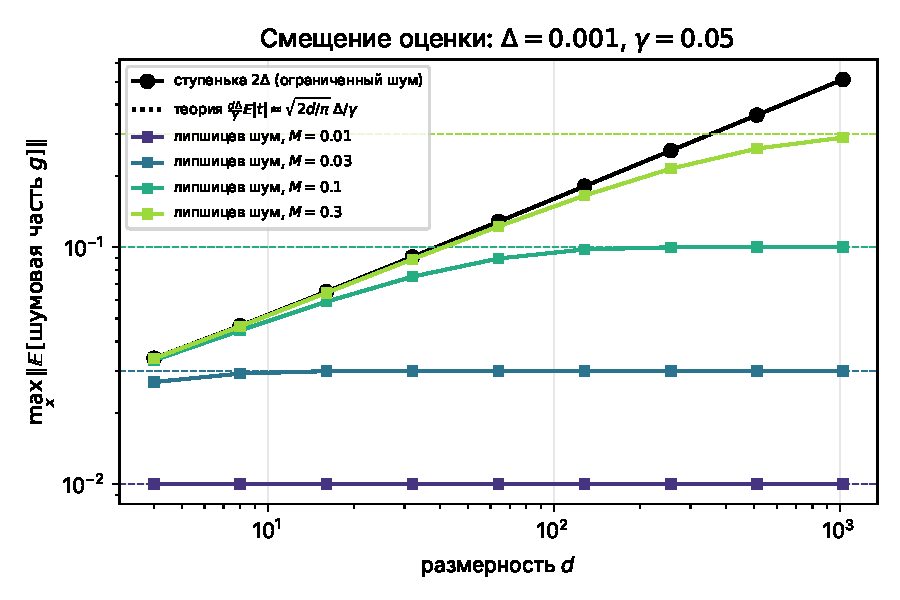
\includegraphics[width=0.49\linewidth]{figures/e1_bias.pdf}\hfill
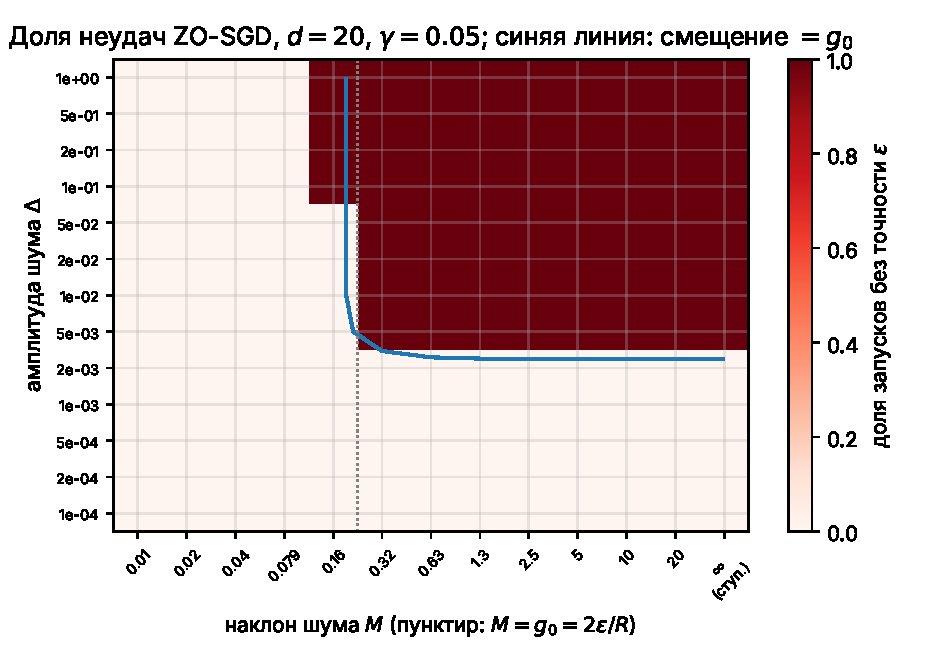
\includegraphics[width=0.49\linewidth]{figures/e2_phase.pdf}
\caption{\textbf{Left:} maximal bias of the two-point estimator, computed by exact quadrature, for a step of height $2\Delta$ (grows as $\sqrt{2d/\pi}\,\Delta/\gamma$) and for ramps of slope $M$ (never exceeds $M$; equals $M$ for $d\ge128$). \textbf{Right:} success of the method against a noise ``wall'' of amplitude $\Delta$ and slope $M$, $d=20$; the prediction ``the method stops iff the bias exceeds the gradient of the problem'' agrees with the experiment in $97.6\%$ of the cells, and the safe region is L-shaped.}
\label{fig:phase}
\end{figure}

\paragraph{Bias versus dimension (\cref{fig:phase}, left).} For $f\equiv0$ and noise depending on one coordinate, the mean of the estimator reduces to a one-dimensional integral with density $\propto(1-t^2)^{(d-3)/2}$, which we compute without Monte Carlo error. The bias of a step matches $\frac{d\Delta}{\gamma}\E|t|$ to $10^{-4}$, growing from $0.034$ ($d=4$) to $0.511$ ($d=1024$); the bias of an $M$-Lipschitz ramp never exceeds $M$.

\paragraph{The theorems at their own constants (\cref{fig:theorems}).} With the parameters of \cref{thm:upper} ($\eps=0.2$, $D=2$, $d\in\{5,10,20,40\}$, $N$ up to $1.9\cdot10^5$) and noise at the limit of \eqref{eq:cond}, the worst error over 8 runs is at most $0.083\eps$: the constants are conservative by about $12\times$. Against the ``counter'' noise of \cref{thm:lower} on a linear objective with gradient $g_0$, the error as a function of $M/g_0$ is the same for $d=5,20,80$, whereas the failure threshold of a bounded step noise moves as $1/\sqrt d$.

\begin{figure}[t]
\centering
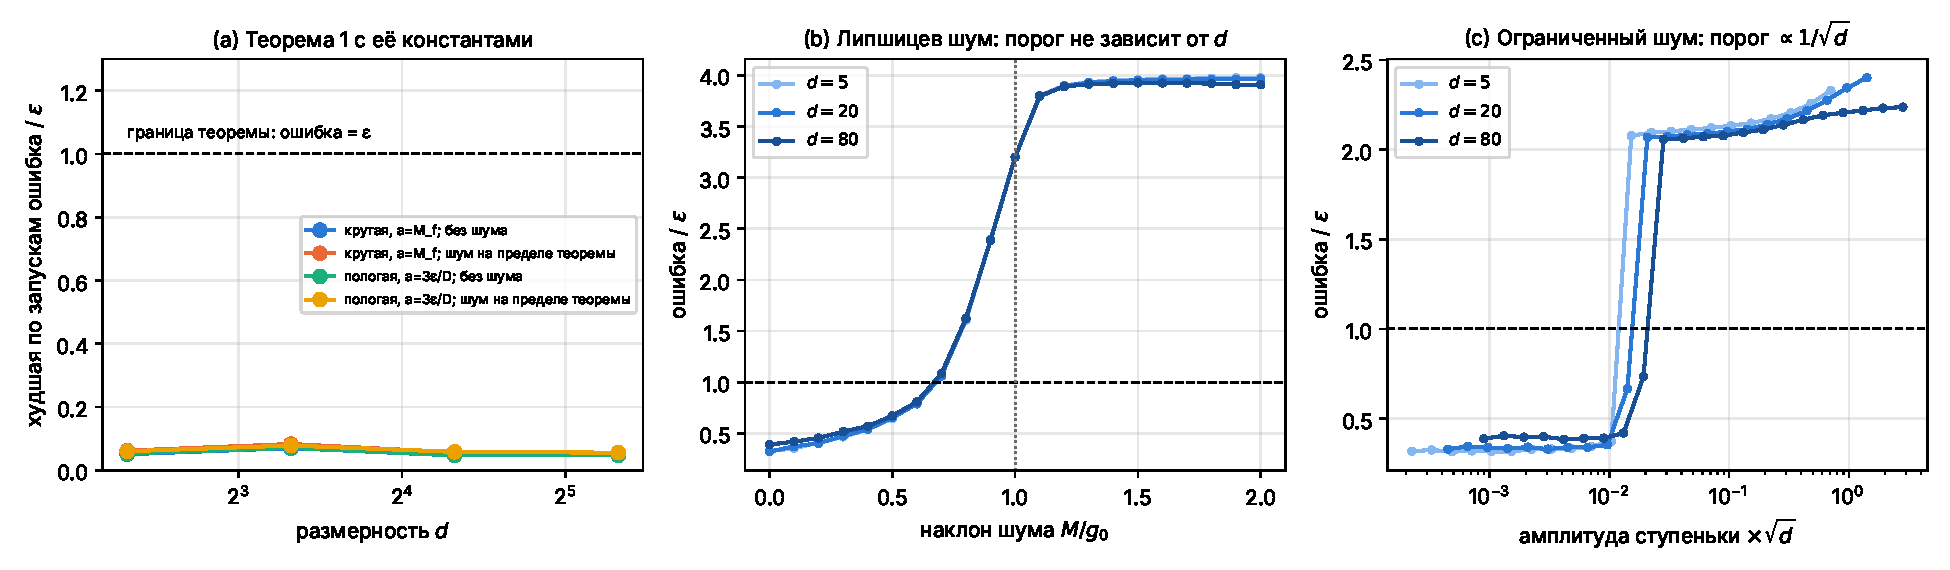
\includegraphics[width=\linewidth]{figures/e4_theorems.pdf}
\caption{\textbf{(a)} Error of \cref{thm:upper} with its own constants, without noise and with noise at the limit of \eqref{eq:cond}. \textbf{(b)} Lipschitz counter-noise: the threshold in $M/g_0$ does not depend on $d$. \textbf{(c)} Bounded step noise: thresholds align in the coordinate $\Delta\sqrt d$, i.e.\ scale as $1/\sqrt d$.}
\label{fig:theorems}
\end{figure}

\paragraph{Floating-point rounding (\cref{fig:rounding}).} We evaluate $f(x)=1+\norm{x-c}_1/\sqrt d$ ($M_f=1$) in fp64, fp32, bf16, fp16, and fp16 with unbiased stochastic rounding. Rounding is far from worst-case: the bound $M_f\gamma+D\sqrt d\,q/(2\gamma)$ is pessimistic by two to three orders of magnitude. For small $\gamma$ the method fails for a different reason: the two rounded values coincide, the estimate is zero, and the iterate does not move. The threshold for bf16 is $8=2^3$ times that for fp16, exactly the difference in mantissa bits, and stochastic rounding moves it down by about $3\times$. Measuring the threshold in fp16 for $d=4,\dots,128$, we find $\gamma_{\mathrm{crit}}\approx0.2\sqrt d\,q/M_f$ (slope $0.49$ in log--log coordinates, predicted $0.5$), in line with the heuristic $|f(x+\gamma e)-f(x-\gamma e)|\approx2\gamma|\ip{\nabla f}e|\sim2\gamma M_f/\sqrt d$.

\begin{figure}[t]
\centering
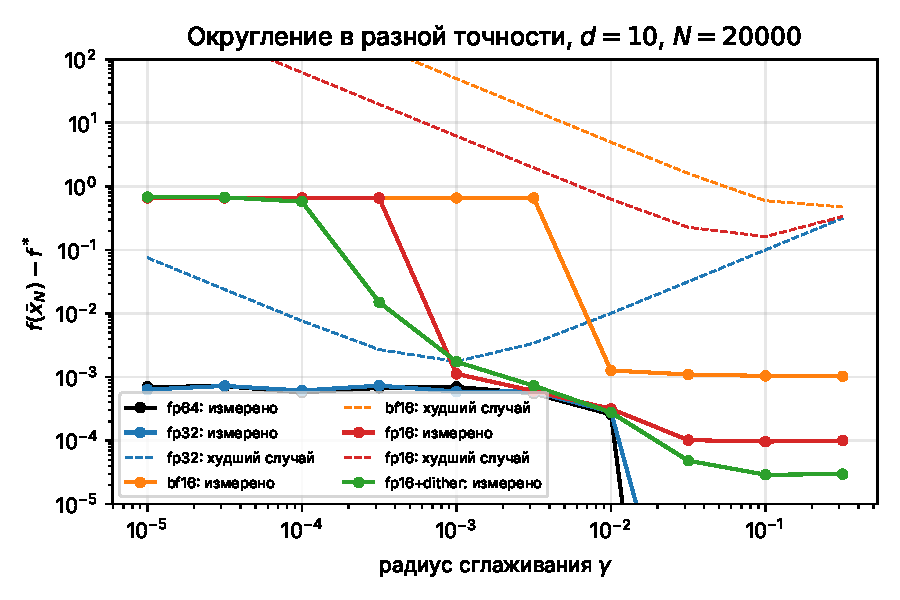
\includegraphics[width=0.49\linewidth]{figures/e3_rounding.pdf}\hfill
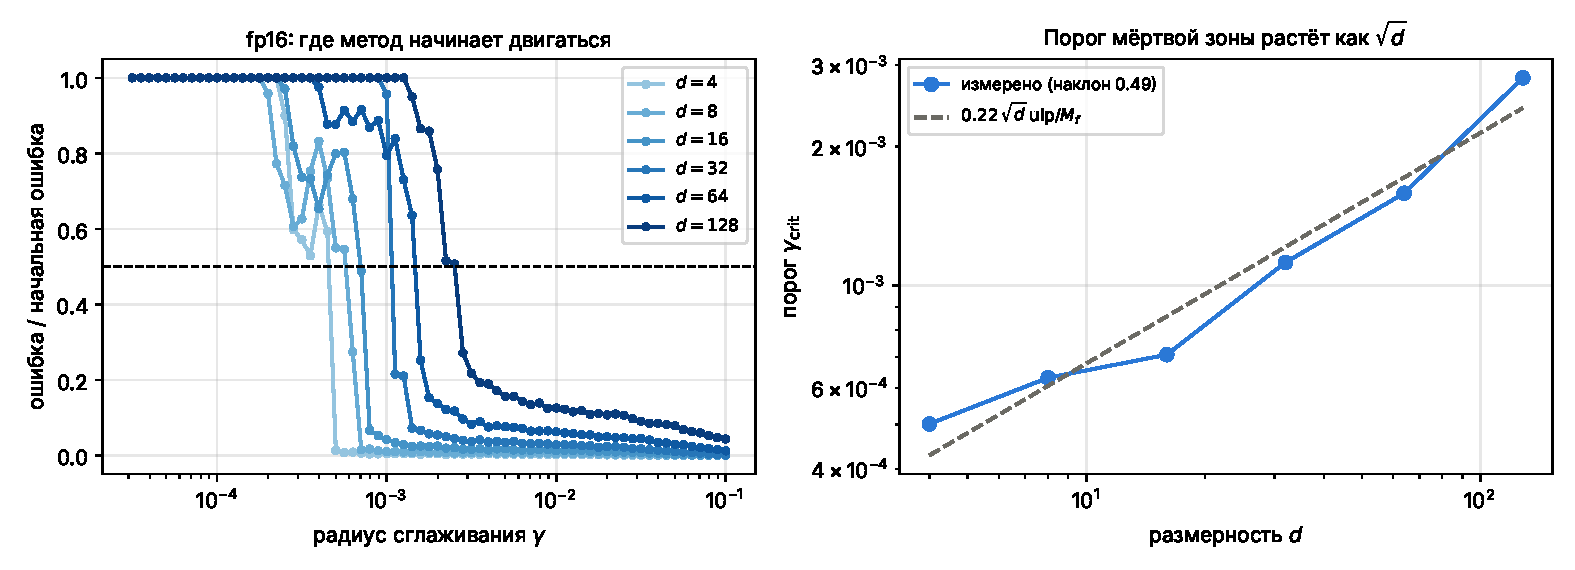
\includegraphics[width=0.49\linewidth]{figures/e5_dead_zone.pdf}
\caption{\textbf{Left:} final error versus smoothing radius for different precisions ($d=10$); dashed: worst-case bound. \textbf{Right:} dead-zone threshold $\gamma_{\mathrm{crit}}$ in fp16 versus $d$; the fitted slope is $0.49$.}
\label{fig:rounding}
\end{figure}

\section{Discussion and limitations}\label{sec:discussion}

\paragraph{Scope.} Our method is non-accelerated; the batched accelerated scheme of \citet{gasnikov2022power} achieves $O(d^{1/4}M_fD/\eps)$ rounds, and whether the threshold $\Theta(\eps/D)$ survives acceleration requires a bias-robustness argument for accelerated methods with bounded iterates, which we do not provide \citep[cf.][]{devolder2014first}. The dead-zone law is empirical.

\paragraph{Open questions.} (i) The motivating example of the conjecture in \citet[Appendix~B]{dvinskikh2022noisy} is the error of a sample average, which is Lipschitz with constant $M/\sqrt n$ on the queried points but only $\sqrt dM/\sqrt n$ globally. Whether $\sqrt d$ is necessary for noise that is Lipschitz \emph{only on the queried points} appears to be open. (ii) A theory of rounding that explains both the dead zone and the gap to the worst case. (iii) Methods that are simultaneously optimal in calls, rounds and admissible Lipschitz noise.

\section*{AI use statement}
This work was carried out with substantial help of a generative AI assistant (a large language model with code execution). The assistant was used for literature search and reading, for drafting and checking proofs, for writing the experiment code and tests, and for drafting the text of this paper. Every lemma is additionally checked numerically by unit tests included in the supplementary material, and the novelty claims were checked against the full texts of the cited papers. \textbf{[Authors: before submission, state here which parts you verified yourselves (e.g., proofs checked line by line, code reviewed) --- do not submit this sentence.]} We take full responsibility for the content of this work.

\section*{Reproducibility statement}
All assumptions are stated in \cref{sec:setup}; complete proofs are given in \cref{app:proofs}. The supplementary material contains the code, a single script that reproduces all figures and tables with fixed random seeds, and the unit tests; experimental parameters are listed in \cref{app:experiments}.

\bibliography{references}
\bibliographystyle{iclr2027_conference}

\appendix

\section{Proofs}\label{app:proofs}

Throughout, $\cF_k=\sigma(e_0,\dots,e_{k-1})$; the point $x_k$ is $\cF_k$-measurable and $e_k$ is independent of $\cF_k$.

\begin{fact}[smoothing; \citealp{flaxman2005online,gasnikov2022survey}]\label{fact:smooth}
If $h$ is continuous, then $h_\gamma(x)=\E_uh(x+\gamma u)$ is differentiable and
$\nabla h_\gamma(x)=\frac d\gamma\E_e[h(x+\gamma e)e]=\frac d{2\gamma}\E_e[(h(x+\gamma e)-h(x-\gamma e))e]$.
If $h$ is $M$-Lipschitz, so is $h_\gamma$, hence $\norm{\nabla h_\gamma}\le M$. If $h$ is moreover convex, $h_\gamma$ is convex and $h\le h_\gamma\le h+\gamma M$.
\end{fact}
The first identity is the divergence theorem on the ball of radius $\gamma$ (the ratio of the area of the sphere to the volume of the ball is $d/\gamma$); the second follows from the symmetry $e\mapsto-e$.

\begin{fact}[sphere; \citealp{ledoux2001concentration}]\label{fact:sphere}
Let $e\sim\unif(S^{d-1})$, $d\ge2$. (a) $\E\ip er^2=\norm r^2/d$, hence $\E|\ip er|\le\norm r/\sqrt d$. (b) If $\varphi$ is $L_\varphi$-Lipschitz on $S^{d-1}$, then $\mathrm{Var}\,\varphi(e)\le L_\varphi^2/(d-1)$.
\end{fact}

\begin{lemma}[projected SGD with biased gradients]\label{lem:sgd}
Let $F$ be convex and differentiable, $x_F^*\in\arg\min_QF$, $x_0\in Q$, and let $g_k$ be $\cF_{k+1}$-measurable with $\E[g_k\mid\cF_k]=\nabla F(x_k)+b_k$, $\norm{b_k}\le B$ and $\E[\norm{g_k}^2\mid\cF_k]\le G^2$ almost surely. Then for $x_{k+1}=\Prj(x_k-hg_k)$,
$\E F(\bar x_N)-F(x_F^*)\le\frac{\norm{x_0-x_F^*}^2}{2hN}+\frac{hG^2}2+BD$.
\end{lemma}
\begin{proof}
Let $r_k=\norm{x_k-x_F^*}^2$. Since projection onto $Q$ is non-expansive and $x_F^*\in Q$, $r_{k+1}\le r_k-2h\ip{g_k}{x_k-x_F^*}+h^2\norm{g_k}^2$. Taking $\E[\cdot\mid\cF_k]$ gives $\E[r_{k+1}\mid\cF_k]\le r_k-2h\ip{\nabla F(x_k)+b_k}{x_k-x_F^*}+h^2G^2$. By convexity $\ip{\nabla F(x_k)}{x_k-x_F^*}\ge F(x_k)-F(x_F^*)$, and $|\ip{b_k}{x_k-x_F^*}|\le BD$ because $x_k,x_F^*\in Q$. Taking full expectations, summing over $k<N$ (the sum telescopes and is at most $r_0$) and dividing by $2hN$ bounds the average of $\E F(x_k)-F(x_F^*)$; Jensen's inequality $F(\bar x_N)\le\frac1N\sum_kF(x_k)$ concludes.
\end{proof}

\begin{proof}[Proof of \cref{lem:decomp}]
Taking $y=x$ gives $\delta_L\le\delta$. By \cref{def:class}, $\delta(y)+M\norm{x-y}\ge\delta(x)-\Delta_0$ for all $y$, so $\delta_L\ge\delta-\Delta_0>-\infty$. An infimum of $M$-Lipschitz functions that is finite at one point is finite everywhere and $M$-Lipschitz. Conversely, if $\delta=\ell+\beta$ with $\ell$ $M$-Lipschitz and $\beta\in[0,\Delta_0]$, then $|\delta(x)-\delta(y)|\le M\norm{x-y}+|\beta(x)-\beta(y)|\le M\norm{x-y}+\Delta_0$.
\end{proof}

\begin{proof}[Proof of \cref{lem:bias}]
Write $\delta=\delta_L+\delta_B$ by \cref{lem:decomp}; $\delta_L$ is continuous and $\delta_B=\delta-\delta_L$ is Borel with values in $[0,\Delta_0]$. Accordingly $g=g_1+g_2$, where $g_1$ is built from the continuous function $f+\delta_L$ and $g_2$ from $\delta_B$.

\emph{Bias.} By \cref{fact:smooth} applied to $f$ and to $\delta_L$, $\E g_1=\nabla f_\gamma(x)+\nabla(\delta_L)_\gamma(x)$ with $\norm{\nabla(\delta_L)_\gamma(x)}\le M$. For a unit $r$, since $|\delta_B(a)-\delta_B(b)|\le\Delta_0$, \cref{fact:sphere}(a) gives $|\ip{\E g_2}r|\le\frac d{2\gamma}\Delta_0\E|\ip er|\le\frac{\sqrt d\Delta_0}{2\gamma}$. Taking the supremum over $r$ and setting $b=\nabla(\delta_L)_\gamma(x)+\E g_2$ gives the bias bound.

\emph{Second moment.} $\norm g^2\le2\norm{g_1}^2+2\norm{g_2}^2$. The function $\varphi(e)=(f+\delta_L)(x+\gamma e)$ is $\gamma(M_f+M)$-Lipschitz on the sphere, $\norm{g_1}^2=\frac{d^2}{4\gamma^2}(\varphi(e)-\varphi(-e))^2$, and $(\varphi(e)-\varphi(-e))^2\le2(\varphi(e)-\E\varphi)^2+2(\varphi(-e)-\E\varphi)^2$. Since $-e$ has the same law as $e$, \cref{fact:sphere}(b) yields $\E\norm{g_1}^2\le\frac{d^2}{4\gamma^2}\cdot\frac{4\gamma^2(M_f+M)^2}{d-1}\le2d(M_f+M)^2$. Finally $\norm{g_2}^2\le\frac{d^2\Delta_0^2}{4\gamma^2}$.
\end{proof}

\begin{proof}[Proof of \cref{thm:upper}]
\emph{Conditional moments.} Since $e_k$ is independent of $\cF_k$, $x_k$ is $\cF_k$-measurable and $\delta$ is fixed, the conditional law of $g_k$ given $\cF_k$ is the law of the estimator of \cref{lem:bias} at $x_k$. Hence $\E[g_k\mid\cF_k]=\nabla f_\gamma(x_k)+b(x_k)$ with
$\norm{b(x_k)}\le\frac{\eps}{6D}+\frac{\sqrt d}{2}\cdot\frac{3M_f}{\eps}\cdot\frac{\eps^2}{9\sqrt dM_fD}=\frac{\eps}{3D}=:B$.
Similarly $\frac{d^2\Delta_0^2}{2\gamma^2}=\frac{d\eps^2}{18D^2}\le\frac{dM_f^2}{18}\le d(M_f+M)^2$ (using $\eps\le M_fD$), so $\E[\norm{g_k}^2\mid\cF_k]\le5d(M_f+M)^2=G^2$.

\emph{SGD.} With $F=f_\gamma$, $\norm{x_0-x_F^*}\le D$ and $h=D/(G\sqrt N)$, \cref{lem:sgd} gives $\E f_\gamma(\bar x_N)-\min_Qf_\gamma\le\frac{DG}{\sqrt N}+BD\le\frac\eps3+\frac\eps3$, because $N\ge45d(M_f+M)^2D^2/\eps^2=9D^2G^2/\eps^2$.

\emph{Back to $f$.} By \cref{fact:smooth}, $f\le f_\gamma$ and $\min_Qf_\gamma\le f_\gamma(x^*)\le f^*+\gamma M_f=f^*+\eps/3$. Adding up gives $\E f(\bar x_N)-f^*\le\eps$.
\end{proof}

\begin{proof}[Proof of \cref{thm:lower}, details]
The interval $(2\eps/D,\min\{M,M_f\}]$ is nonempty because $M>2\eps/D$ and $M_f>2\eps/D$. The functions $f_\pm$ are convex and $a$-Lipschitz with $a\le M_f$, and $\delta_\pm$ are $a$-Lipschitz with $a\le M$, so $\delta_\pm\in\cN(M,0)$. As the oracle returns $f_\pm+\delta_\pm\equiv0$, the joint law of all queries, answers and the output is the same under both instances, and one of the two expected errors exceeds $\eps$.
\end{proof}

\begin{proof}[Proof of \cref{prop:adaptive}]
(a) The proof of \cref{thm:upper} used only that, conditionally on $\cF_k$, the noise is a fixed function of class $\cN(M,\Delta_0)$ independent of $e_k$; \cref{lem:bias} applies conditionally (joint measurability allows freezing $\cF_k$). (b) $\delta_k$ is $M$-Lipschitz, and at $x_k\pm\gamma e_k$ it equals $\pm\gamma M\sign\ip{e_k}v$. Hence the noise part of the estimator is $dM\sign\ip{e_k}v\,e_k$, whose mean is $dM\,\E|\ip ev|\,v$ by symmetry, and $d\,\E|\ip ev|=d\,\Gamma(d/2)/(\sqrt\pi\,\Gamma((d+1)/2))\sim\sqrt{2d/\pi}$.
\end{proof}

\section{Experimental details}\label{app:experiments}

\paragraph{Bias versus dimension.} $f\equiv0$; noise $\delta(x)=\varphi(x_1)$ with a step $\varphi(z)=\Delta\sign z$ or a ramp $\varphi(z)=\Delta\clip(Mz/\Delta,-1,1)$; $\Delta=10^{-3}$, $\gamma=0.05$, $M\in\{0.01,0.03,0.1,0.3\}$, $d$ from $4$ to $1024$; maximum over the offset $s\in[-2\gamma,2\gamma]$ of the point from the jump. The mean of the estimator is a one-dimensional integral over $t=\ip{e}{e_1}$ with density $\propto(1-t^2)^{(d-3)/2}$, computed on a grid of $4\cdot10^5$ points.

\paragraph{Phase diagram.} $f(x)=-g_0\ip ux$ on the unit ball with $g_0=2\eps$, $\eps=0.1$; noise: a ramp of amplitude $\Delta$ and slope $M$ across $\ip ux=0$ (a step for $M=\infty$); start $x_0=-0.6u$, $d=20$, $\gamma=0.05$, $3000$ iterations, $16$ runs per cell on a $13\times13$ grid. Disagreements with the prediction occur only next to the boundary $M\approx g_0$, where the total slope is small and the method is slowed down rather than stopped; with $10^4$ iterations all runs in that column succeed.

\paragraph{Theorems.} (a) $\eps=0.2$, unit ball ($D=2$), $M_f=1$, parameters exactly as in \cref{thm:upper}; objectives $a\norm{x-c}$ with $\norm c=0.5$ and $a\in\{M_f,3\eps/D\}$; noise $M\ip ux+\Delta_0\mathbb 1[\ip ux>0]$ at the limit of \eqref{eq:cond}; $d\in\{5,10,20,40\}$, $N$ from $23{,}257$ to $186{,}050$, $8$ runs. (b) Linear objective as in the phase diagram, noise $M\ip ux$, $M/g_0\in[0,2]$, $d\in\{5,20,80\}$, $4000$ iterations. (c) Same objective, step noise $\Delta\sign\ip ux$ with $22$ values of $\Delta$ in $[10^{-4},0.3]$.

\paragraph{Rounding.} $f(x)=1+\norm{x-c}_1/\sqrt d$, $d=10$, ball of radius $2$, $2\cdot10^4$ iterations, $6$ runs, $10$ values of $\gamma$ in $[10^{-5},0.3]$. bf16 is emulated by rounding fp32 results to 8 mantissa bits; stochastic rounding rounds the exact value up or down to the fp16 grid without bias. Dead zone: fp16, $q=2^{-10}$, $d\in\{4,\dots,128\}$, $71$ values of $\gamma$ in $[3\cdot10^{-5},0.1]$, $3000$ iterations, $6$ runs; $\gamma_{\mathrm{crit}}$ is the smallest $\gamma$ for which the method at least halves the initial error. Measured $\gamma_{\mathrm{crit}}M_f/(\sqrt dq)$: $0.26, 0.23, 0.18, 0.20, 0.20, 0.26$ for $d=4,8,16,32,64,128$.

\end{document}
